\documentclass[../thesis/thesis.tex]{subfiles}
\begin{document}
 \chapter{Evaluation}
 \label{chap:evaluation}

In this chapter we devise a set of experiments to test the sensor system's properties and come to conclusions as to their effect on our ability to detect occupants. We then outline a process for taking raw sensor data and performing occupancy predictions with it. Using that process, we then devise a set of occupancy scenarios and test the ability of different machine learning algorithms to determine occupancy from that data.

\section{Sensor Properties}

In order to best utilize the \mlx, we must first understand the properties it exhibits and their potential effects on our ability to perform occupancy measurements. These properties can be broadly separated into three different categories: Bias, Noise and Sensitivity.

\subsection{Bias}
When detecting no infra-red radiation (IR), the sensor should indicate a near-zero temperature, as the sensor's method of determining temperature involves measuring IR. If in such conditions the temperatures indicated are non-uniform, that suggests that the sensor has some level of bias in its measurements. We attempted to investigate the possibility of such bias by performing thermal captures of the night sky. While this does not completely eliminate the IR, it does remove a significant proportion of it.

To test this, the thermal sensor was exposed to the night sky at a capture rate of 1~Hz for 4 minutes, with the sensing results combined to create a set of means and standard deviations for the pixels at ``rest''. The average temperature detected was $11.78~\dc$, with the standard deviation remaining less than $0.51~\dc$ over the entire exposure period. The resultant mean and standard deviation thermal maps (\Fref{fig:meanplot} and \Fref{fig:stdplot}) shows that the four centre pixels maintain a similar temperature around $9~\dc$, with temperatures beginning to deviate as they became further from that point.

The most likely cause of bias is related to the physical structure of the sensor. The \mlx is a rectangular sensor which has been placed inside a circular tube. Due to this physical arrangement, the sides of this rectangular sensor will be significantly closer to these edges than the centre. If the sensor's casing is at an ambient temperature higher than the measurement data (as is likely in this case) thermal radiation from the sensor package itself could be significant enough to cause the edges to appear warmer than the observed area of the sky. This effect could be controlled for by cooling the sensor package to below that of the ambient temperature being measured. However, we determine this is not necessary in our project, as the method of calculating a thermal background will compensate for any such bias provided it remains relatively constant, which we predict it should.

\begin{figure}
\centering
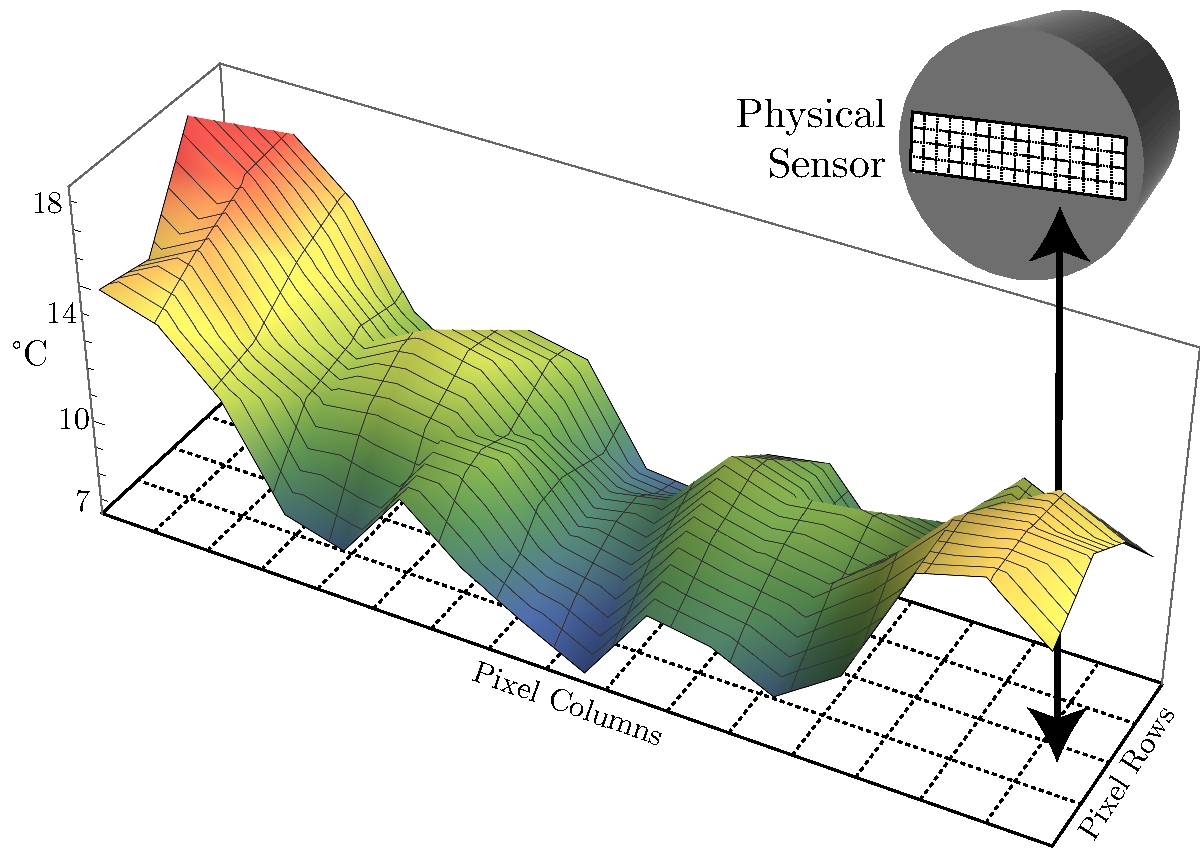
\includegraphics[width=\textwidth]{../diagrams/rest-avg-embed.pdf}
\caption{Mean values of 4 minute night sky thermal capture plotted over sensor's $16\times4$ grid}
\label{fig:meanplot}
\end{figure}

\begin{figure}
\centering
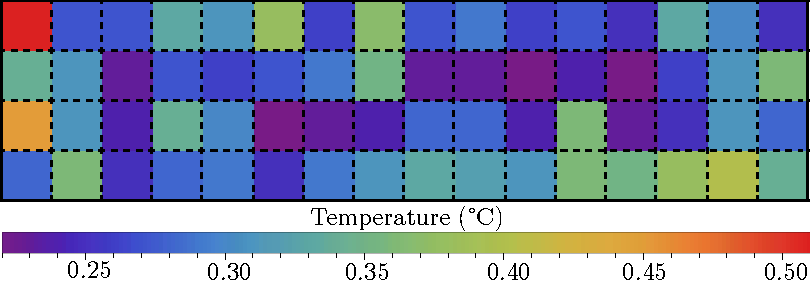
\includegraphics[width=\textwidth]{../diagrams/stddev-contour2.pdf}
\caption{Standard deviation of 4 minute night sky thermal capture plotted over sensor's $16\times4$ grid}
\label{fig:stdplot}
\end{figure}


\subsection{Noise}

One of the primary features of the \mlx is the ability to sample the thermal data at a variety of sample rates between 0.5~Hz and 512~Hz. It was noted in preliminary experimentation that a higher sample rate appeared to result in noisier temperature readings. As our experiments focus on separating occupants from a thermal background, it is important to determine if this noise could affect our ability to reliably separate occupants from the thermal background.

\Fref{fig:noise} plots one of the central pixels of the sensor in a scenario where it is detecting a background, and when it is viewing a person, at the five different sample rates achievable with the current hardware configuration. We can see in these plots that the data becomes significantly more noisy as the sample rate increases, and we can also conclude that the sensor uses a form of data smoothing at lower sample rates, as the variance in data increases with sample rate. If the sample rate was to increase beyond a certain threshold, it is likely that the ability for the sensing system to disambiguate between objects of interest and the background would diminish.

\begin{figure}
  \centering
  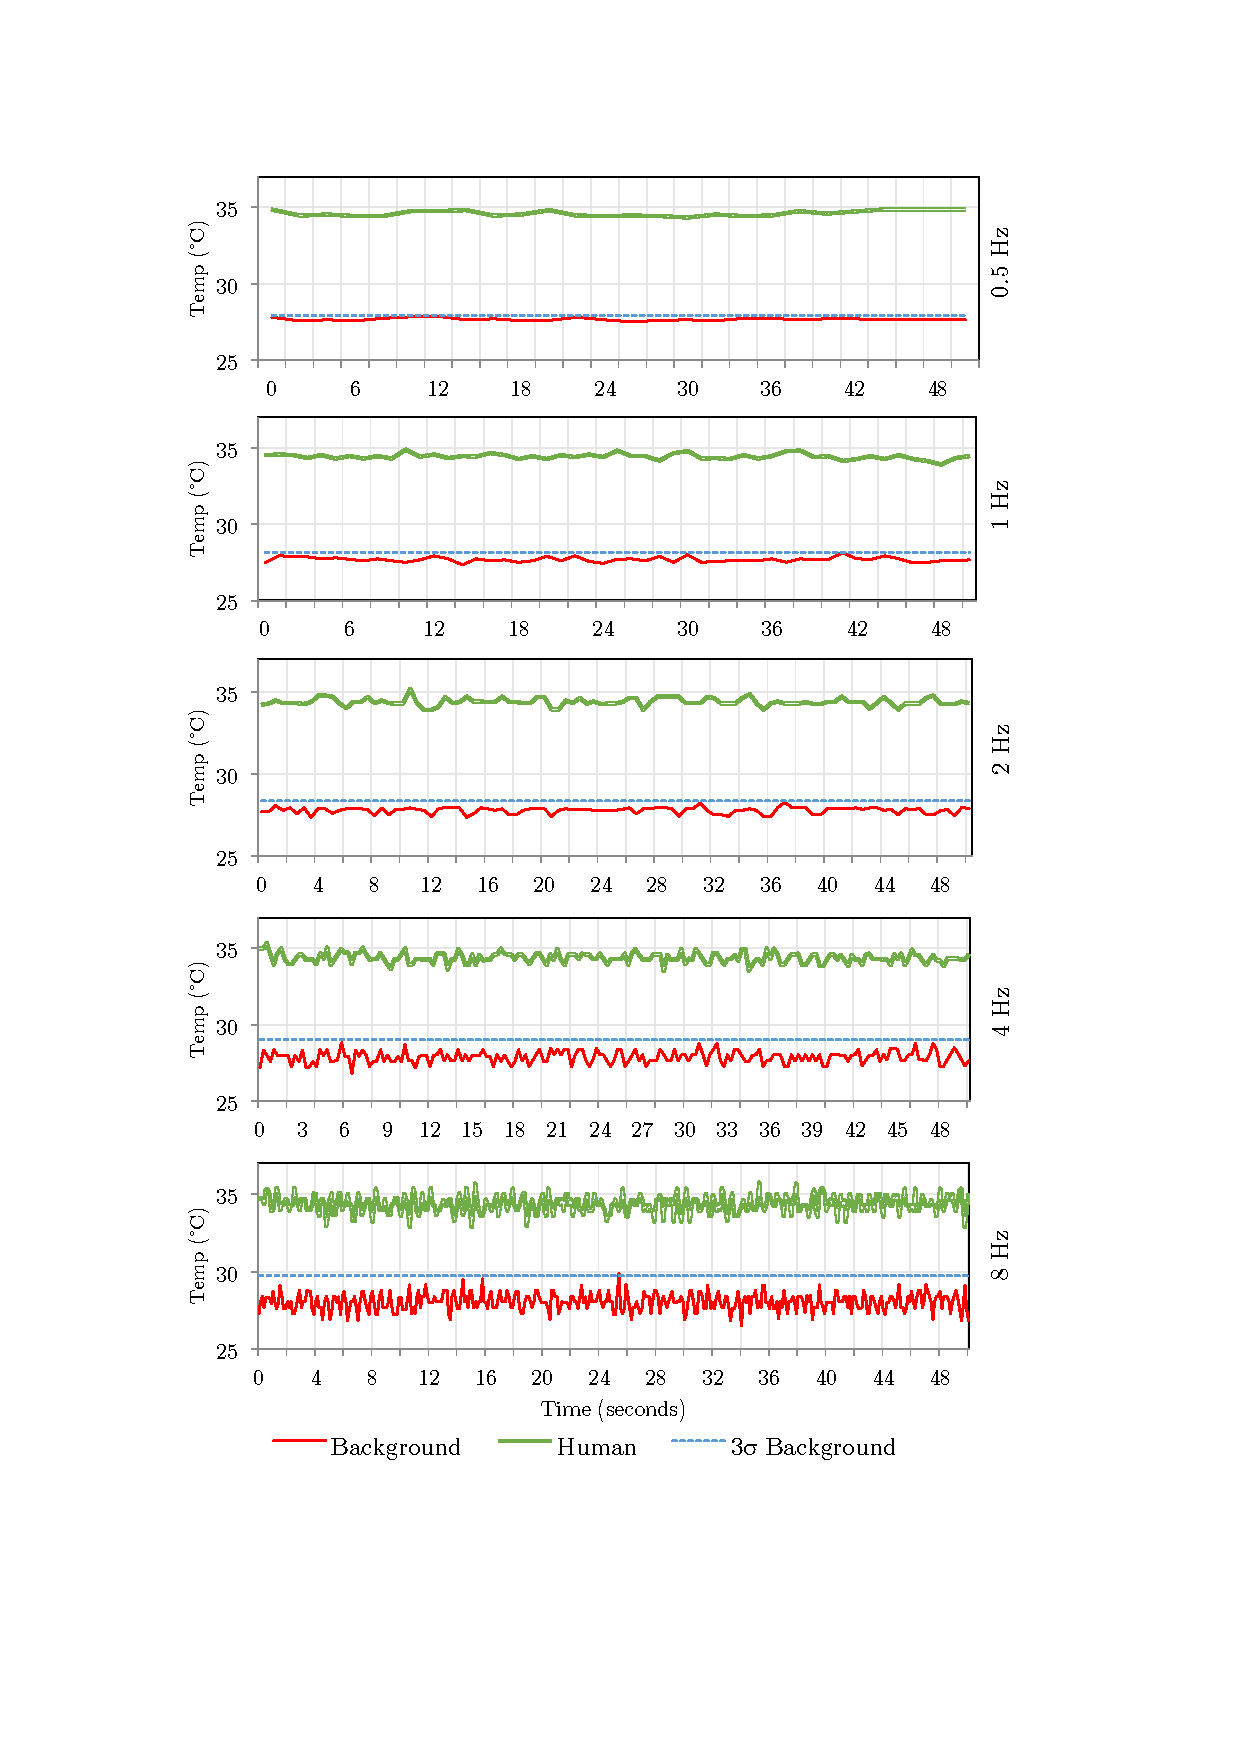
\includegraphics[width=0.9\textwidth]{../diagrams/noise-graph4.pdf}
  \caption{Plot of occupant and background sensor noise at sampling speeds 0.5~Hz -- 8~Hz}
  \label{fig:noise}
\end{figure}

In the 0.5~Hz case, the third standard deviation above background ($3\sigma$) is $6.4~\dc$ below the minimum occupant value ($o$) detected. As the noise increases, this gap slowly decreases, with $5.75~\dc$ for 1~Hz, $5.53~\dc$ for 2~Hz, $4.48~\dc$ for 4~Hz, and finally $3.15~\dc$ for 8~Hz. In none of these cases is $3\sigma \ge \mathrm{min}(o)$, which would completely rule that sample rate out.

Based on the data, noise will not pose any issue as the slowest sampling rate of 0.5~Hz is sufficient for the system's needs, and shows a sufficiently large gap between occupant and background temperatures.

\subsection{Sensitivity}
\label{subsec:sensitivity}

The \mlx is a sensor composed of 64 independent non-contact digital thermopiles, which measure infra-red radiation to determine the temperature of objects. While they are bundled in one package, the sensor's block diagram discussed previously (\Fref{fig:exps:blockdia}) shows that they are in fact wholly independent sensors placed in a grid structure. This has important effects on the properties of the data that the \mlx produces. 

\Fref{fig:hotmotion} shows a smoothed temperatures graph of six of the sensor's central pixels as a hot object is moved from left to right at an approximately constant speed. One of the most interesting phenomena in this graph is the variability of the object's detected temperature as it moves ``between'' two different pixels; there is a noticeable drop in the objects detected temperature. Each pixel appears to exhibit a bell-curve like line, with the detected temperature increasing from the baseline and peaking as the object enters the centre of the pixel, and the detected temperature similarly decreasing as the object leaves the centre. 

This phenomenon has several possible causes. One likely explanation is that each individual pixel detects objects radiating at larger angles of incidence to be colder than they actually are. As the object enters a pixel's effective field of view, it will radiate into the pixel at an angle that is at the edge of the pixel's ability to sense, with this angle slowing decreasing until the hot object is directly radiating into the pixel's sensor, causing a peak in the temperature reading. As the object leaves the individual element's field of view, the same happens in reverse.

This phenomena is not anticipated to impact our intended use case, as it only strongly affects objects at pixel or sub-pixel size. In our experimental conditions the sensor will not be sufficiently distant that humans could be detected as such sizes.

\begin{figure}
\centering
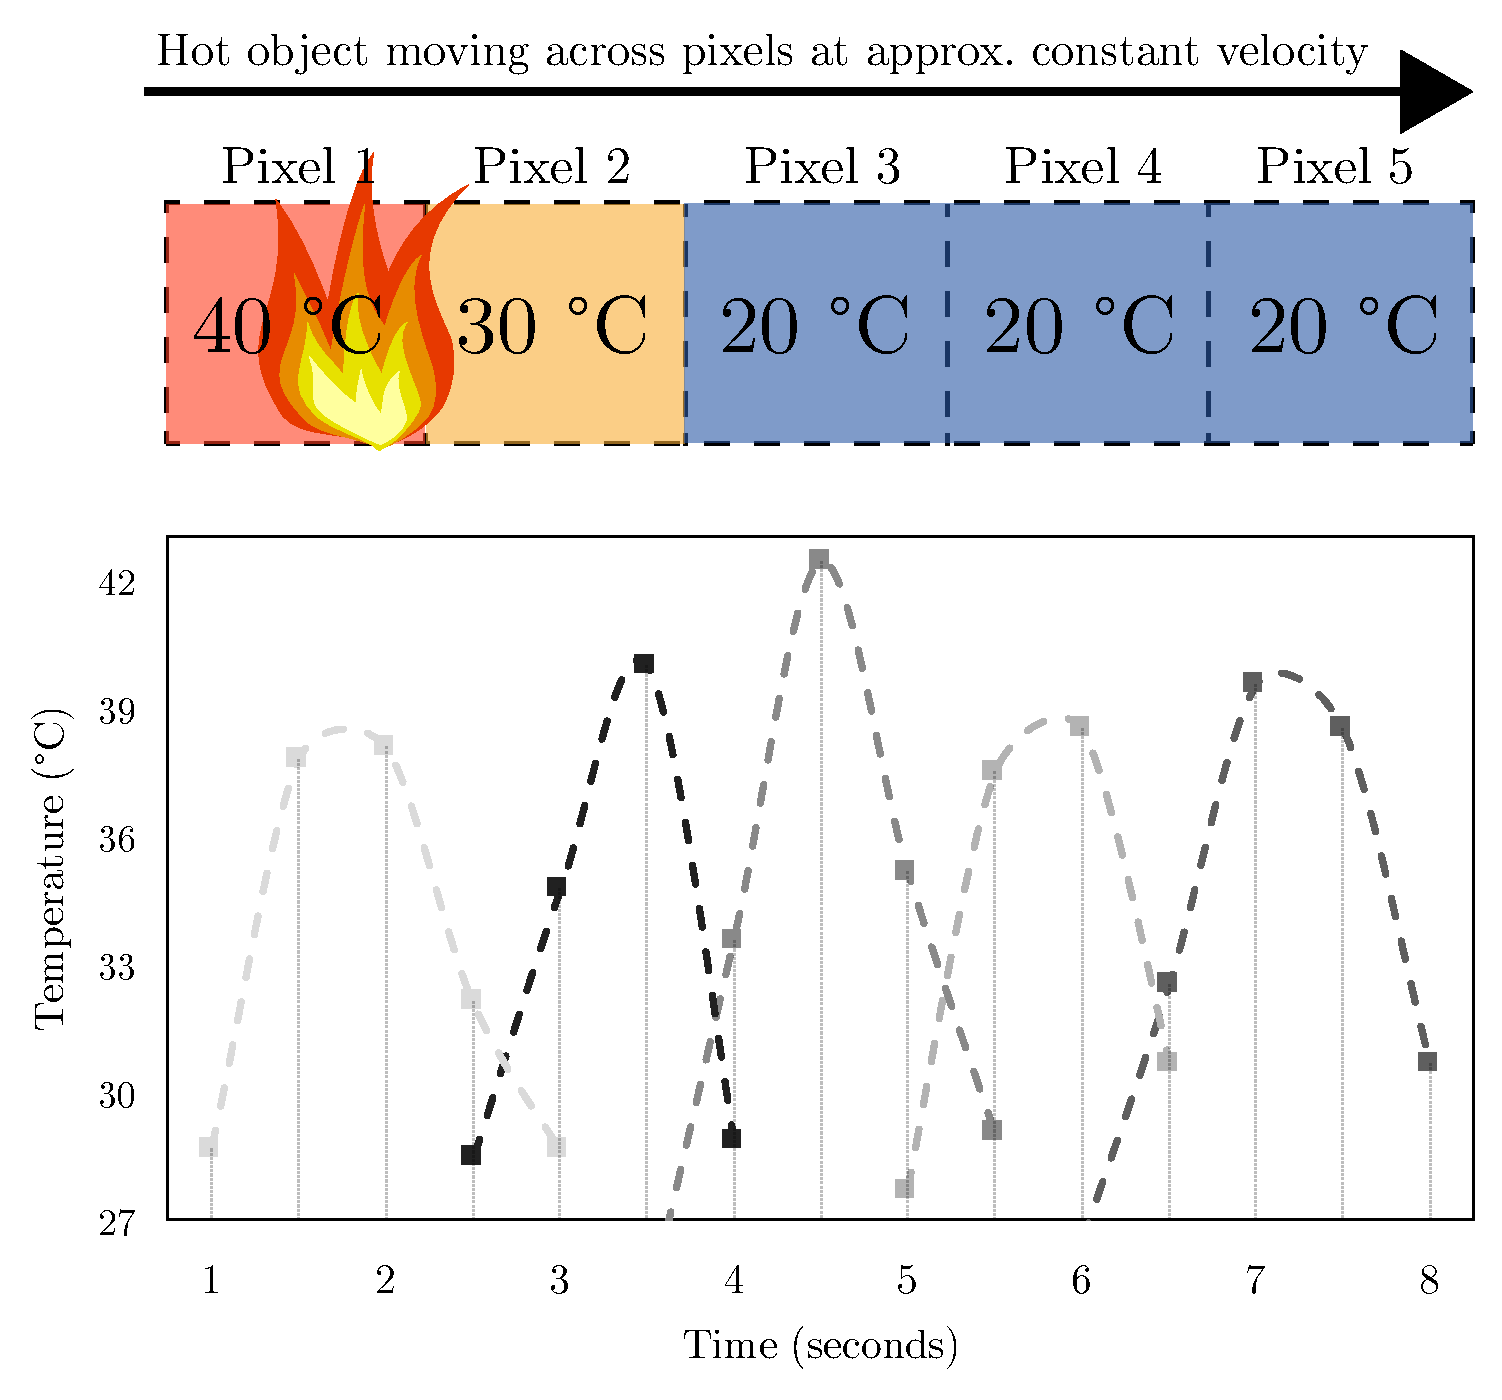
\includegraphics[width=\textwidth]{../diagrams/03_hot_water_top_row_modified2.pdf}
\caption{Temperature plot of five of the MLX90620's pixels as a hot object moves across them at a constant velocity}
\label{fig:hotmotion}
\end{figure}

\clearpage{}

\section{Classification}
With deeper understanding of the prototype's caveats, it is now possible to proceed to the data collection stage. Both thermal and visual data can be collected determine the effectiveness of the machine learning classification algorithms used. Due to the prototype's technical similarly to ThermoSense~\cite{beltran2013thermosense}, a similar set of experimental conditions will be used, with a comparison against ThermoSense being used as a benchmark. To this end, several experiments were devised, each of which had its data gathered and processed in accordance with the same general process, outlined in \Fref{fig:methods:flowchart} and discussed in more detail in this section.

\begin{figure}
\centering
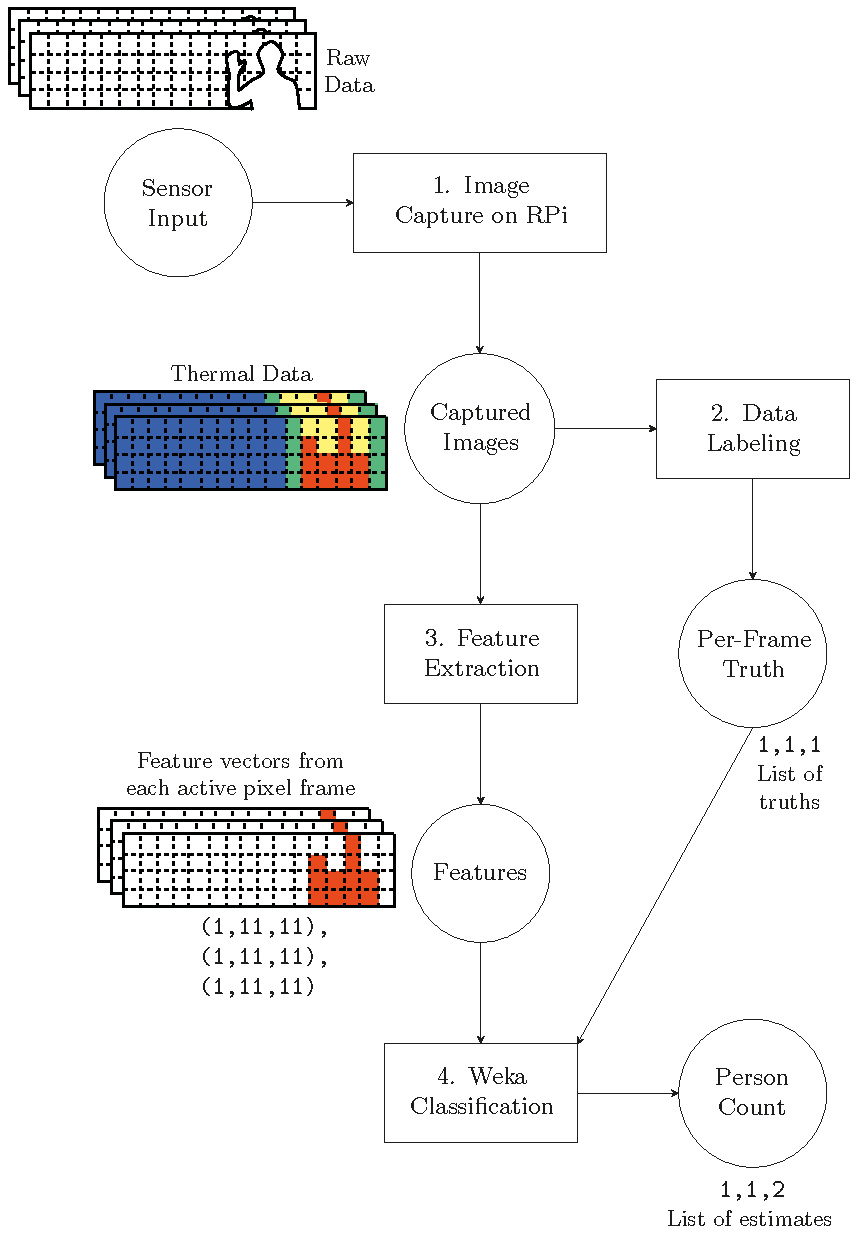
\includegraphics[width=0.97\textwidth]{../diagrams/process-pics.pdf}
\caption{Process flow diagram for turning raw sensor input into occupancy estimates}
\label{fig:methods:flowchart}
\end{figure}

\subsection{Data Collection}
As the camera and the Arduino are directly plugged into the Raspberry Pi, all data capture is performed on-board through SSH, with the data being then copied off the Pi for later processing. To perform this capture, the main script used is \texttt{cap\_pi\_synced.py}.

\texttt{cap\_pi\_synced.py} takes two parameters on the command line; the name of the capture output, and the number of seconds to capture. The script initializes the \texttt{picamera} library, then passes a reference to it to the \texttt{capture\_synced} function within the \texttt{Visualizer} class. The class will then handle sending commands to the Arduino to capture data in concert with taking still frames with the Raspberry Pi's camera.

When the script runs, it creates a folder with the name specified, storing the thermal capture inside a file named \texttt{output\_thermal.hcap} and a sequence of files with the format \texttt{video-\%09d.jpg} corresponding to each visual capture frame.

\subsection{Data Labelling}
\label{subsec:datalabelling}
Once this data capture is complete, the data is copied to a computer with GUI support for labelling. The utility \texttt{tagging.py} is used for this stage. This script is passed the path to the capture directory and the number of frames at the beginning of the capture that are guaranteed to contain no motion. This utility will display frame by frame each visual and thermal capture together, as well as the computed feature vectors (based on a background map created from the first $n$ frames without motion).

The user is then required to press one of the number keys on their keyboard to indicate the number of people present in this frame. This number will be recorded in a file called \texttt{truth} in the capture's directory. The next frame will then be displayed, and the process continues. This utility enables the quick input of the ground truth of each capture, which is necessary for the classification stage.

\subsection{Feature Extraction and Data Conversion}
Once the ground truth data is available, it is now possible to utilize the data to perform various classification tests. For this, we use version 3.7.12 of the open-source Weka toolkit~\cite{Weka}, which provides easy access to a variety of machine learning algorithms and the tools necessary to analyse their effectiveness.

We collate and export the ground truth and extracted features from multiple captures to a Comma Seperated Value (CSV) file for processing with Weka. \texttt{weka\_export.py} takes two parameters, a comma-separated list of different experiment directories to pull ground truth and feature data from, and the number of frames at the beginning of each capture that can be considered as ``motionless.'' With this information, a CSV-file file is generated.

\subsection{Executing Weka Tests}
Once the CSV file is generated, it is then possible to process this file through Weka. Weka provides a variety of machine learning classification algorithms to choose from. To investigate ThermoSense's results, we replicate their algorithmic implementations in Weka. We discuss the general theory behind of each of these algorithms in Appendix \ref{chap:appendix:classification}. In total, Thermosense uses three machine learning classifiers:

Firstly, they use an Artificial Neural Network with a hidden layer of five neurons, with a sigmoid activation function for the hidden layer and a linear activation function for the output layer. They test only the one, two and three person cases, relying on their \pir to detect the zero person case. They use 70\% of their data for training the neural net, 15\% for testing the net and the final 15\% for validating their results. ThermoSense conducts tests interpreting the number of people as a numeric attribute.

We use Weka's ``MultilayerPerceptron'' neural network to recreate this, which creates a hidden layer of $((\mathrm{attributes} + \mathrm{classes}) / 2)$ (in our case three neurons) by default, however we manually reconfigure this to be one hidden layer of five neurons, like ThermoSense. It uses a sigmoid activation function for all neurons, except in the case that a numerical answer is to be predicted, in which case, like ThermoSense, it uses a linear activation function for the output layer.

Secondly, they use a $k$-Nearest Neighbours (KNN) where $k=5$, with the distance between features being determined by their Euclidean distance. For determining the class label, higher weightings are given to training points inversely to their distance from the point being classified.

Weka's ``iBk'' function is used to perform a KNN calculation, configuring \texttt{distanceWeighting} to be ``Weight by 1-distance'' and \texttt{KNN} to be 5, to make the classification as similar in function to the ThermoSense approach as is possible. ThermoSense does not specify what validation technique they used, so we elected to use a 10-fold cross-validation.

Thirdly, they use a Linear Regression model of $y = \beta_A A + \beta_S S + \beta $, whereby $A$ is the number of active pixels, $S$ is the size of the largest connected component, and the $\beta$ values represent the corresponding coefficients. They opt to exclude the third feature, the number of connected components, as their testing indicates that excluding it minimizes the Root Mean Squared Error (RMSE) further. 

We use Weka's ``LinearRegression'' function, and exclude the number of connected components (\texttt{numconnected}) attribute from the feature vector list, as ThermoSense does, to attempt to match this approach.

In addition to the above three techniques, we use our own techniques (included in \Fref{tab:methods:params}). Our techniques are predominately common in use, with their general theory described in Appendix \ref{chap:appendix:classification}. One algorithm that isn't as common that we have chosen is the KStar (K*) algorithm, which we describe in further detail here:

The K* algorithm, developed by Cleary and Trigg~\cite{cleary1995k} presents a different approach to $k$-nearest Neighbours type algorithms. With K* the distance used to compare similar points is not the Euclidean distance, but rather an entropic distance, a measure of how much effort is required to convert one example into another. This has several positive effects; it makes the algorithm more robust to missing values and enables the classifier to output either a numeric or nominal result.

We decided to use K* as one of our classification algorithms as it presents an interesting and different approach to more commonly used algorithms, and also allows the investigation of KNN-like techniques in the numeric area. K* is present in Weka as ``KStar,'' and we will opt to use it in its default state.

\begin{table}
\centering
\begin{tabular}{|p{40mm}|p{20mm}|p{70mm}|}
\hline
\textbf{Type} & \textbf{Attribute} & \textbf{Weka Class} \& \textbf{Parameters} \\ \hline

{Neural Network \newline (ANN)} & {Nominal, \newline Numeric} & \texttt{weka.classifiers.functions\newline.MultilayerPerceptron \newline -L 0.3 -M 0.2 -N 500 -V 15 \newline -S 0 -E 20 -H 5} \\ \hline

{$k$-nearest Neighbours \newline (KNN)} & Nominal, \newline Numeric & \texttt{weka.classifiers.lazy.IBk \newline -K 5 -W 0 -F \newline -A "weka.core.neighboursearch\newline.LinearNNSearch -A \textbackslash"weka.core\newline.EuclideanDistance \newline -R first-last\textbackslash""} \\ \hline

Naive Bayes & Nominal & \texttt{weka.classifiers.bayes.NaiveBayes} \\ \hline

{Support Vector \newline Machine (SVM)} & Nominal & \texttt{weka.classifiers.functions.SMO \newline -C 1.0 -L 0.001 -P 1.0E-12 \newline -N 0 -V -1 -W 1 \newline -K "weka.classifiers.functions\newline.supportVector.PolyKernel \newline-C 250007 -E 1.0"} \\ \hline

{C4.5 \newline Decision Tree} & Nominal & \texttt{weka.classifiers.trees.J48 \newline -C 0.25 -M 2} \\ \hline

K* & Nominal, \newline Numeric & \texttt{weka.classifiers.lazy.KStar \newline -B 20 -M a} \\ \hline

Linear Regression & Numeric & \texttt{weka.classifiers.functions\newline.LinearRegression \newline -S 0 -R 1.0E-8} \\ \hline

0-R & Nominal, \newline Numeric & \texttt{weka.classifiers.rules.ZeroR} \\ \hline
\end{tabular}
\caption{Weka parameters used for different classifications algorithms}
\label{tab:methods:params}
\end{table}

To help maximize the efficiency of the classification tasks, we use the Weka's Knowledge Flow interface, which provides a drag-and-drop method of creating complex input and output schemes involving multiple different pre-processing steps and classification algorithms. We generate an encompassing flow that accepts an input CSV file of the raw data, and performs all numeric and nominal classification at once, returning a text file with the results of each of the different classification techniques run. The Knowledge Flow's structure can be seen in Appendix \ref{chap:knowledgeflows}. To further automate this a Jython script, \texttt{run\_flow.py} is used to call the flow through Weka's Java API. After this is complete, the script then runs a series of regular expressions on the output text data to generate a summary CSV file with the relevant statistical values.

For those tests that are ``nominal,'' the number of people ground-truth attribute (\texttt{npeople}) was interpreted as nominal using the ``NumericToNominal'' filter, which creates a class for each value detected in \texttt{npeople}'s columns and thus causes nominal occupancy predictions. For those tests that are ``numeric,'' \texttt{npeople} is left unchanged, as by default all CSV import attributes are interpreted as numeric, thus causing numeric occupancy predictions. For all tests where not specifically stated otherwise, we use 10-fold cross-validation to validate our results.

As the data we are using is based on real experiments, the number of frames which are classified as each class may be unbalanced, which could in turn cause a bias in the classification results. We found that in most cases, the data that most unbalanced the set was that of the zero case, as it was the case most present in the data. As ThermoSense previously demonstrated, the use of the \pir alone allows for determining the zero/not-zero case effectively without classification algorithms. Due to this, we rebalance our dataset by excluding all zero cases from the data Weka receives.

\subsection{Classifier Experiment Set}
In our first set of experiments, a scene was devised in accordance with \Fref{fig:exps:3setup} that attempted to sense people from above, as did ThermoSense. The prototype was set up on the ceiling, pointing down at a slight angle to both prevent the interference of the mounting pole (see \Fref{fig:pictures:protoact}) and to increase thermal mass detected. For ease of use, the prototype was powered by mains power, and had the Raspberry Pi networked with a laptop for command input and data collection via Ethernet. This set of experiments involved between one and three people being present in the scene, moving in and out in various ways in accordance with the following scripts.

The first four sub-experiments involved people standing;
\begin{itemize}
\item Sub-exp 1: One person walks in, stands in centre, walks out of frame.
\item Sub-exp 2: One person walks in, joined by another person, both stand there, one leaves, then another leaves.
\item Sub-exp 3: One person walks in, joined by one, joined by another, all three stand there, one leaves, then another, then another.
\item Sub-exp 4: Two people walk in simultaneously, both stand there, both leave simultaneously.
\end{itemize}

The latter five sub-experiments involved people sitting;
\begin{itemize}
\item Sub-exp 5: One person walks in, sits in centre, moves to right, walks out of frame.
\item Sub-exp 6: One person walks in, joined by another person, both sit there, they stand and switch chairs, one leaves, then another leaves.
\item Sub-exp 7, 8: One person walks in, joined by one, joined by another, they all sit there, one leaves, one shuffles position, then another leaves, then another. (x2)
\item Sub-exp 9: Two people walk in, both sit there simultaneously, both leave simultaneously.
\end{itemize}

In these experiments people moved slowly and deliberately, making sure there were large pauses between changes of action. When not otherwise specified, all people entered from the left and exited from the right. The people involved were of average height, wearing various clothing. The room was cooled to 18 degrees for these experiments.

Each experiment was recorded with a thermal-visual synchronisation at 1~Hz over approximately 60-120 second intervals. Each experiment had 10-15 frames at the beginning where nothing was within the view of the sensor to allow the thermal background to be calculated. Each frame generated from these experiments was manually tagged with the ground truth value of its number of occupants using the tagging script discussed in \Fref{subsec:datalabelling}. A breakdown of the number of frames collected for each occupancy type can be found in \Fref{tab:expbreak}.

The resulting features and ground truth were combined and exported to CSV allowing Weka to analyse them. This data was analysed with the feature vectors always being considered numeric data and with the ground truth considered both numeric and nominal.

\begin{table}
\centering
\begin{tabular}{|r|r|r|r|}
\hline
\textbf{Occupants} & \textbf{Instances} & \textbf{\% (incl. 0)} & \textbf{\% (excl. 0)} \\ \hline
0                  & 444                & 42.2                  &                       \\ \hline
1                  & 252                & 24.0                  & 41.5                  \\ \hline
2                  & 291                & 27.7                  & 47.9                  \\ \hline
3                  & 64                 & 6.1                   & 10.5                  \\ \hline
Total              & 1051               & 100.0                 & 100.0                 \\ \hline
\end{tabular}
\caption{Breakdown of experimental data by occupant ground truth}
\label{tab:expbreak}
\end{table}

 \begin{figure}
 \centering
 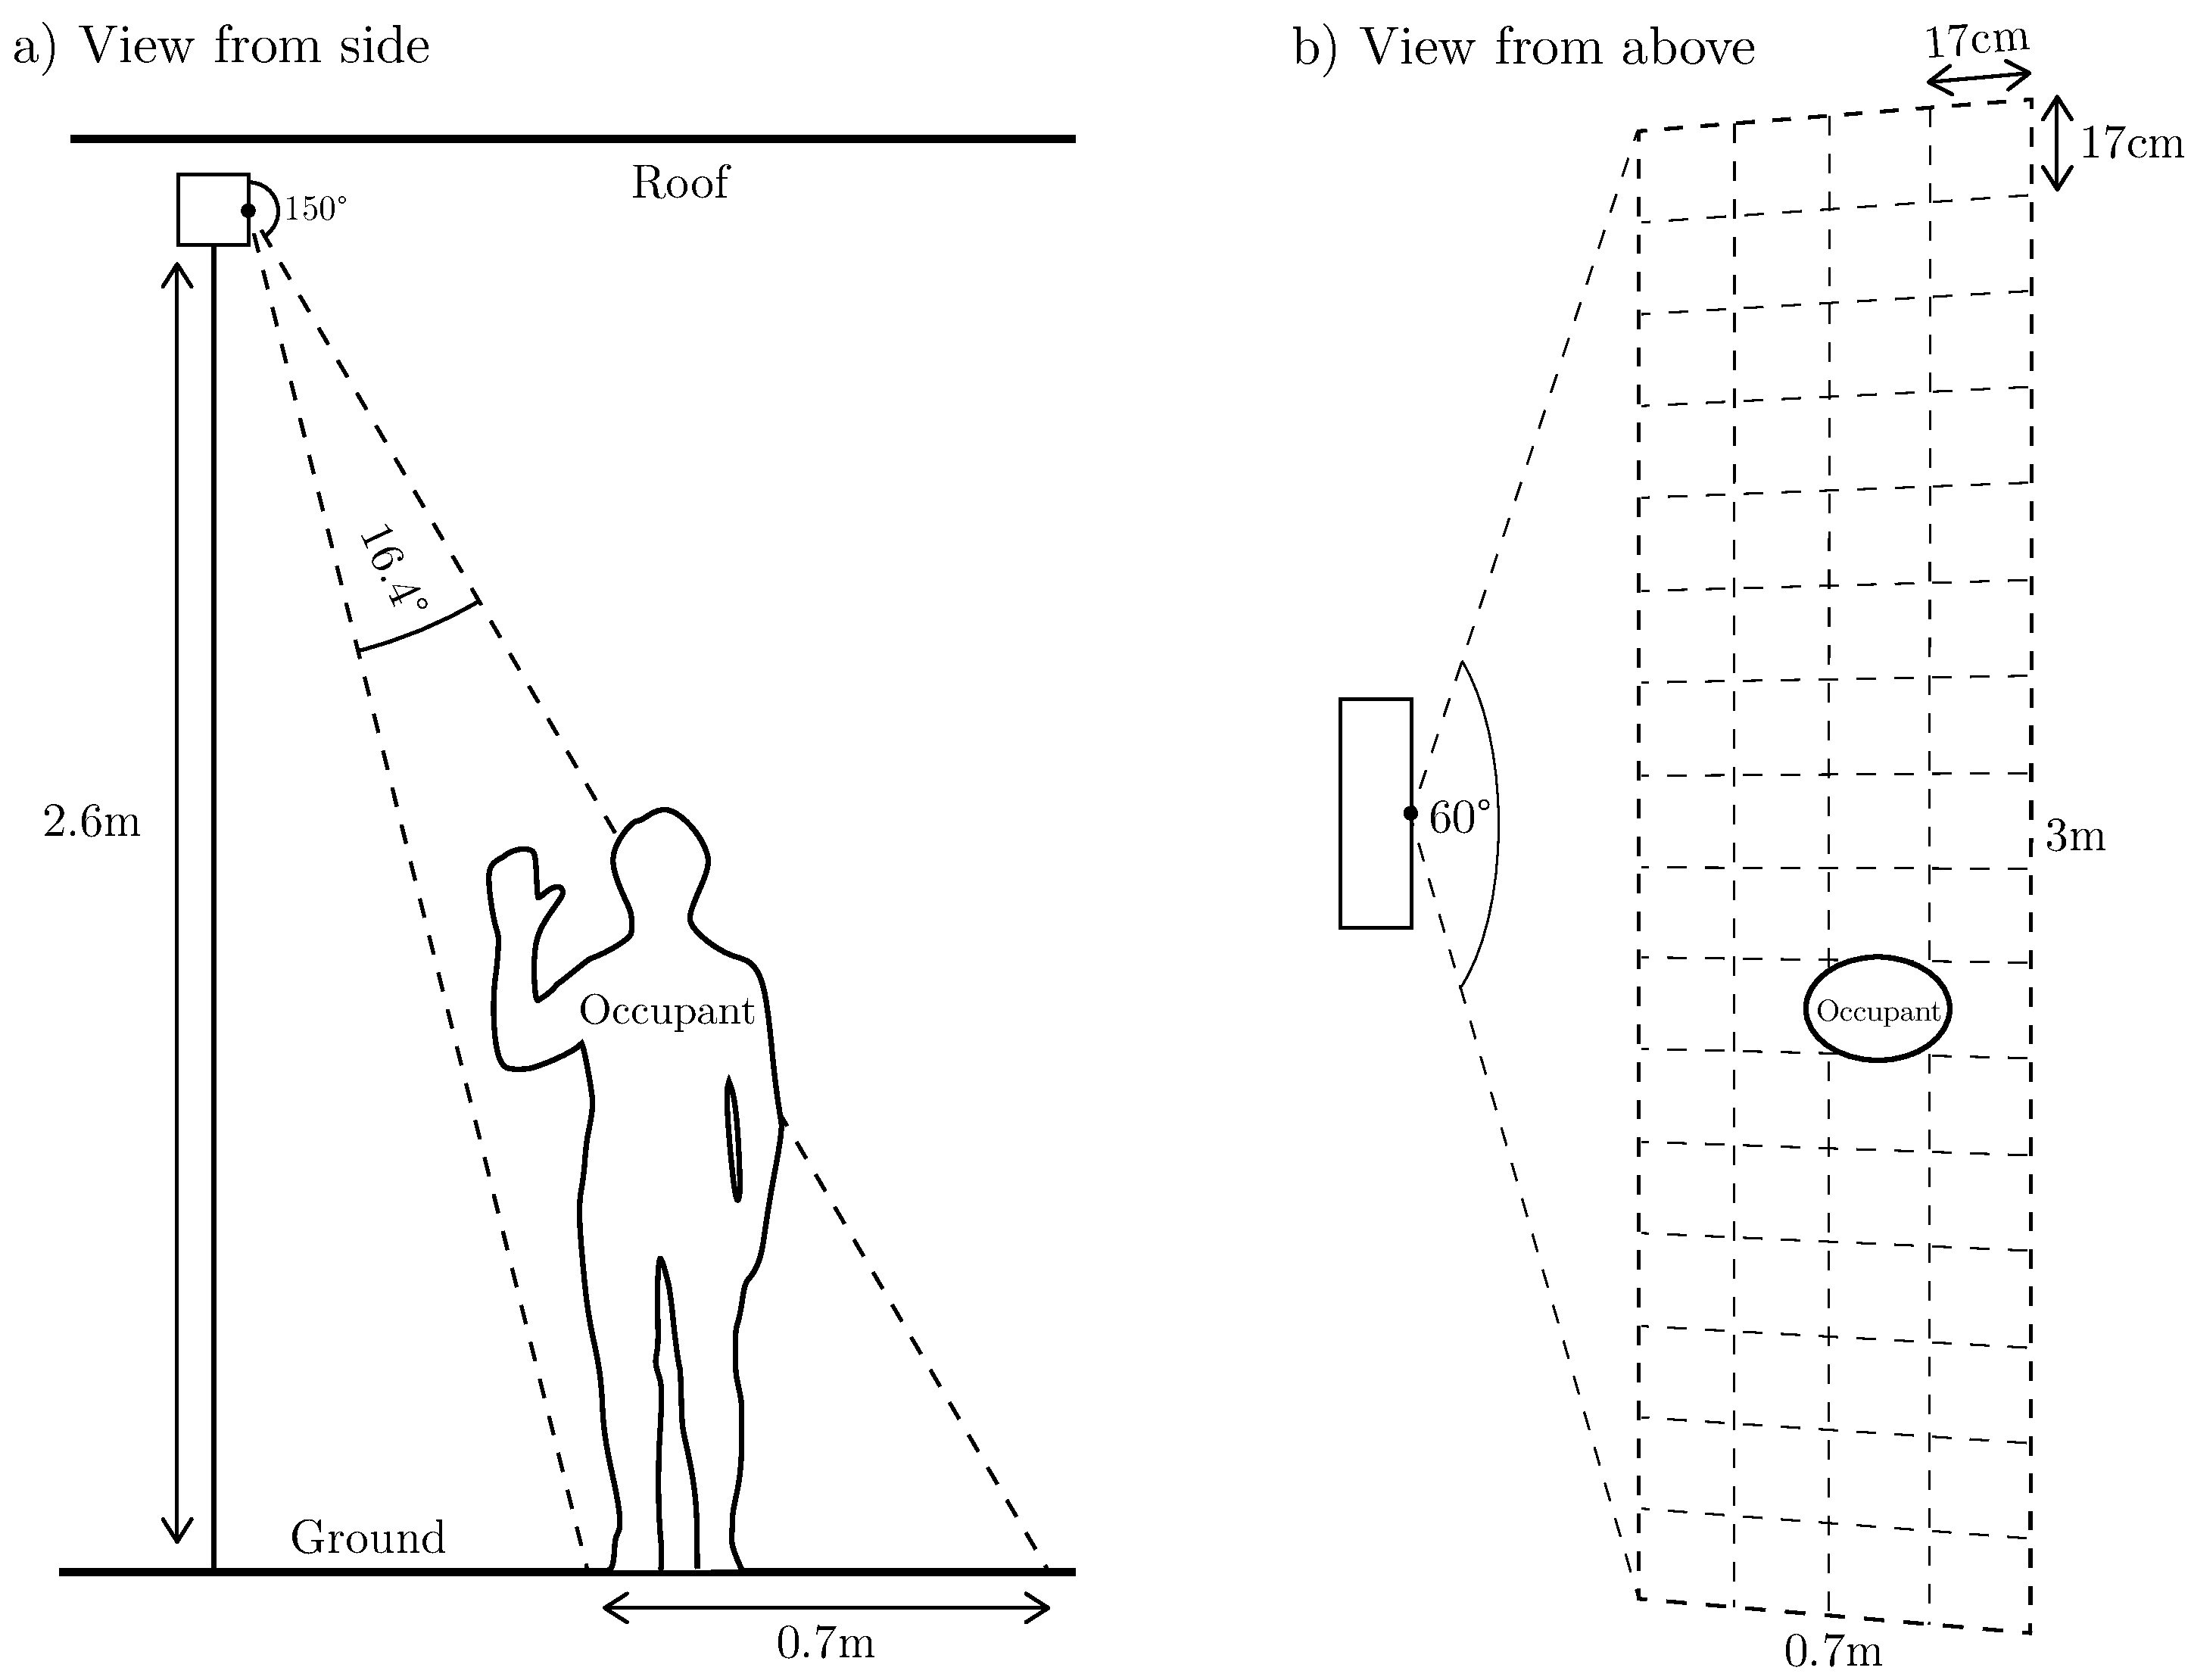
\includegraphics[width=\textwidth]{../diagrams/third-exp-setup2.pdf}
 \caption{Classifier Experiment Set Setup (measurements approximate)}
 \label{fig:exps:3setup}
 \end{figure}

 \clearpage{}

\section{Results}
\label{sec:results}

\subsection{Classification}
\label{subsec:classification}

\begin{table}
\centering
\begin{tabular}{|l|r|r|r|}
\hline
\textbf{Classifier} & \textbf{RMSE} & \textbf{Precision (\%)} & \textbf{Correlation ($r$)} \\ \hline
\multicolumn{4}{|c|}{\cellcolor{black!15} ThermoSense Actual}                         \\ \hline
KNN$^1$             & 0.346         &             &              \\ \hline
Lin Reg$^2$         & 0.385         &             & 0.926        \\ \hline
MLP                 & 0.409         &             & 0.945        \\ \hline
\multicolumn{4}{|c|}{\cellcolor{black!15} ThermoSense Replication}                    \\ \hline
KNN (Nom)$^1$       & 0.364         & 65.65       &              \\ \hline
MLP                 & 0.592         &             & 0.687        \\ \hline
Lin Reg$^2$         & 0.525         &             & 0.589        \\ \hline
KNN (Num)$^1$       & 1.123         &             & 0.377        \\ \hline
\multicolumn{4}{|c|}{\cellcolor{black!15} Numeric}                                    \\ \hline
K*                  & 0.423         &             & 0.760        \\ \hline
0-R                 & 0.651         &             & -0.118       \\ \hline
\multicolumn{4}{|c|}{\cellcolor{black!15} Nominal}                                    \\ \hline
K*                  & 0.304         & 82.56       &              \\ \hline
C4.5                & 0.314         & 82.39       &              \\ \hline
MLP                 & 0.362         & 77.14       &              \\ \hline
SVM                 & 0.398         & 67.18       &              \\ \hline
N. Bayes            & 0.405         & 63.59       &              \\ \hline
0-R                 & 0.442         & 49.74       &              \\ \hline
\end{tabular}\\
\parbox{300pt}{
$^1$: Includes zero occupant cases in training data \\
$^2$: Excludes number of connected components feature \\
\%: Precision, measuring a nominal test result \\
$r$: Correlation coefficient, measuring a numeric test result \\
}
\caption{Results of Classification Experiment Set classification replicating ThermoSense algorithms and using self-selected algorithm}
\label{tab:results:set1}
\end{table}

Significant care was taken to ensure that the same classification parameters were used between our experiments and those performed in ThermoSense to provide as accurate as possible a comparison between our results. However, there were some ambiguities with the ThermoSense results that have made it more difficult to determine which parameters to choose. In particular, with reference to the $k$-Nearest Neighbours tests (KNN), it was ambiguous within the ThermoSense paper as to if they had elected to use a nominal classification or a numeric classification for this data.

Because of this, four tests were performed overall to replicate the ThermoSense results as closely as possible; KNN tests for both numeric and nominal representations of data, a Multi-Layer Perceptron numeric test (MLP) and a Linear Regression numeric test (Lin Reg). With these tests we found that our prototype did not achieve comparable results. ThermoSense reported correlation coefficients ($r$) of around 0.9 for their MLP and Lin Reg tests, however we could not replicate these results, with our best being 0.69 and 0.59 respectively. We were also unable to replicate the low Root Mean Squared Errors (RMSEs) reported by ThermoSense, with their RMSEs for KNN, MLP and Lin Reg being 0.346, 0.385 and 0.409 respectively, while ours were 0.364 (KNN Nominal Case), 1.123 (KNN Numeric Case), 0.592 (MLP) and 0.525 (Lin Reg). Our numeric KNN test performed worse than the 0-R benchmark for numeric tests, indicating an exceedingly poor classification result, with it achieving an RMSE of 1.123 vs. the 0-R's 0.651.

For our own proposed nominal classification algorithms, our accuracies were significantly improved, and in some cases exceeded the RMSEs reported by ThermoSense. Within our dataset, the K* and C4.5 algorithms were most accurate, with accuracies of 82.56\% and 82.39\% respectively. They both achieved RMSEs lower than the best achieved by ThermoSense, with their 0.304 and 0.314 a significant improvement on ThermoSense's KNN RMSE of 0.346.

Following down the ranking, our nominal MLP performed next best, with an accuracy of 77.14\%, and an RMSE of 0.362, which is slightly higher than ThermoSense's best result. Following, the Support Vector Machine (SVM) implementation achieved a relatively poor accuracy of 67.18\% with an RMSE of 0.398, and finally the Naive Bayes (N. Bayes) approach, achieved the worst accuracy of 63.59\% with an RMSE of 0.405. None of these techniques however achieved an RMSE or accuracy worse than our 0-R benchmark, which achieved an RMSE of 0.442 and an accuracy of 49.74\%.

In our sole numeric choice of K*, we found that it achieved a better correlation than any replicated ThermoSense technique, with $r = 0.760$. Additionally, its RMSE of 0.423 was also superior.

\clearpage{}

\subsection{Energy Efficiency}
\label{subsec:energy}

\begin{table}
\centering
\begin{tabular}{|c|c|r|r|}
\hline
\multicolumn{2}{|c|}{\textbf{Connected}} & \multicolumn{2}{c|}{\textbf{Power}} \\ \hline
\textbf{MLX}           & \textbf{PIR}           & \textbf{mA}         & \textbf{V}         \\ \hline
\cmark                 & \cmark                 & 52                  & 4.92               \\ \hline
\cmark                 & \xmark                 & 52                  & 4.92               \\ \hline
\xmark                 & \cmark                 & 46                  & 4.92               \\ \hline
\xmark                 & \xmark                 & 46                  & 4.92               \\ \hline
\multicolumn{2}{|c|}{Power Saving$^1$}          & 34                  & 4.92               \\ \hline
\end{tabular}\\
\parbox{260pt}{
$^1$: \texttt{SLEEP\_MODE\_PWR\_DOWN} AVR mode on Arduino\\
MLX: \mlx\\
PIR: \pir
}
\caption{Energy consumption of sensing system in aggregate and per component}
\label{tab:results:energy}
\end{table}

A YZXStudio USB 3.0 Power Monitor was used to measure power consumed by the Pre-Processing and Sensing tier together while experimenting, as in a more advanced prototype, they would be envisioned to be run on battery power. This was done by connecting the Arduino's USB cable to the Monitor, and the Monitor to a computer. It was calculated (see \Fref{tab:results:energy}) that the average power consumption was 52~mA at 4.92~volts with a sample rate of 0.5~Hz, while continuously outputting data over USB Serial. This power consumption did not vary measurably between sample rates.

To determine the draw from the \pir and \iar, we disconnected all sensors from the Arduino, and ran the power measurement again. The same code was run on the Arduino. This time we received a result of 46~mA  for all sample rates. We found that this power consumption appeared to be from the \mlx, as adding/removing the \pir had negligible effects on power consumption. Power consumption also did not appear to vary depending on the temperature of the objects being detected, or the motion properties of the scene. We can then conclude that the sensors themselves draw around 6~mA of current.

We also ran the Arduino in the most aggressive power saving mode available on the hardware, and measured how much power was consumed with and without sensors attached. It appears that this power saving mode disables all sensor power, as in both cases a draw of 34~mA was measured. This represents a saving of 12~mA from the base Arduino current consumption.

\section{Discussion}

\subsection{Classification}
As discussed in \Fref{subsec:classification} our prototype achieves positive results. However, our results indicate that there is a fundamental difference between our set of experiments and those performed by ThermoSense. None of our attempts to replicate their results succeeded, with every replicated result performing significantly worse than that of ThermoSense. The most likely reason for this is that the differences in the field of view of the \mlx when compared to the Grid-EYE is significant enough to affect the suitability of the algorithms used. In particular the \mlx created far more instances of partial people within the sensed region. This presents a key caveat for any future researchers attempting to reapply ThermoSense's methodology to a different sensor.

With the specific classification techniques that we choose to test, we found significant variation in their success. Our best techniques, K* and C4.5, were highly similar in result and with a significant gap to the third-best technique, the Multi-Layer Perceptron. It is notable that both K* and C4.5 use entropy measures to make decisions, we hypothesise that their use of entropy is related to their accuracy.

Examining the plots of the Euclidean distance for the features (\Fref{fig:featplots}), it is apparent there is no obvious separation between the different classes, with the three sets of values overlapping significantly. This explains $k$-Nearest Neighbours (KNN) and Support Vector Machine's (SVM) poor performance with our data.

In the case of KNN, a selection of the nearest neighbours may not be indicative of the feature vector's class membership. A similar idea applies in the case of SVM, the aforementioned plots suggest that there may be no clear hyperplane through which the different classes of data can be separated.

The success of entropy-based methods suggests that the separation of classes is less of an issue when distance is measured with entropy, as in the case of K*, or when entropy is used to divide the dataset, as in the case of C4.5. In \Fref{fig:correctplots} we can see a comparison of the predictions of the SVM algorithm against that of K*. For the central part of the graph (20 $<$ Active pixels $<$ 35), the predictive power of both algorithms appears similar. However in the left and right parts of the graph, we can see that SVM fails to correctly separate the classes. This suggests that SVM's use of support vectors to split the feature space is ill-suited to the overlapping features of the dataset, and that K*'s entropy-based approach is able to find more suitable splits.

Due to the white box nature of decision trees, it is possible for us to further example the tree generated by the C4.5 algorithm  to determine how sensible the branches are. We can see from \Fref{lst:tree} that C4.5 considers the number of active pixels to be the strongest indicator of the number of occupants. This makes intuitive sense, as the number of active pixels should be the most general descriptor of the number of occupants. This is followed by the size of largest connected component, and the number of connected components. Overall the decisions made by the C4.5 tree appear sensible, although in some places it appears the tree had few cases to form branches with, which could be rectified with an increase in the size of the dataset.

Our worst selected technique was Naive Bayes. It is not unusual that it performed so poorly, as the ``Naive'' part of the technique is an assumption of independence between the different features input, which is clearly false with our features. All three of our features relate to the same underlying graph and are most definitely correlated with each other.

By using the K* or C4.5 machine learning algorithm, we are confident that the prototype could achieve appropriate levels of accuracy for its occupancy goals.

\begin{listing}

%TC:ignore
\begin{minted}[fontsize=\footnotesize,frame=single]{text}
# numactive: Number of active pixels in frame
# sizeconnected: Number of active pixels in largest connected component
# numconnected: Number of connected components in frame

# Leaf format:
# <attribute name> <comparator> <value>:
#     <classified as class>
#     (<total number of instances reaching leaf>
#     /<number of those instances that are misclassified>)
# e.g. attribute <= 10: 3 (100.0/50.0)

# Fractional measures are caused by the distribution of samples with
# missing values

numactive <= 20
|   sizeconnected <= 10
|   |   numactive <= 10
|   |   |   numconnected <= 2
|   |   |   |   numactive <= 9
|   |   |   |   |   numactive <= 5
|   |   |   |   |   |   numactive <= 4: 1 (22.96/5.6)
|   |   |   |   |   |   numactive > 4: 2 (16.0/3.0)
|   |   |   |   |   numactive > 5
|   |   |   |   |   |   sizeconnected <= 5: 2 (2.0)
|   |   |   |   |   |   sizeconnected > 5: 1 (67.0/6.0)
|   |   |   |   numactive > 9: 2 (22.0/3.0)
|   |   |   numconnected > 2: 1 (20.0)
|   |   numactive > 10: 2 (68.0/6.0)
|   sizeconnected > 10: 1 (132.04/22.4)
numactive > 20
|   sizeconnected <= 24
|   |   numactive <= 36
|   |   |   sizeconnected <= 15: 2 (144.0/17.0)
|   |   |   sizeconnected > 15
|   |   |   |   numactive <= 22
|   |   |   |   |   numactive <= 21
|   |   |   |   |   |   numconnected <= 1: 1 (3.0/1.0)
|   |   |   |   |   |   numconnected > 1: 3 (2.0)
|   |   |   |   |   numactive > 21: 1 (2.0)
|   |   |   |   numactive > 22: 2 (44.0/14.0)
|   |   numactive > 36: 3 (12.0/4.0)
|   sizeconnected > 24
|   |   numconnected <= 1: 2 (4.0/2.0)
|   |   numconnected > 1: 3 (24.0/2.0)
\end{minted}
%TC:endignore

\caption{C4.5 Decision tree generated by Weka's J48 implementation from the Classification Experiment Set data}
\label{lst:tree}
\end{listing}

\begin{figure}
\centering
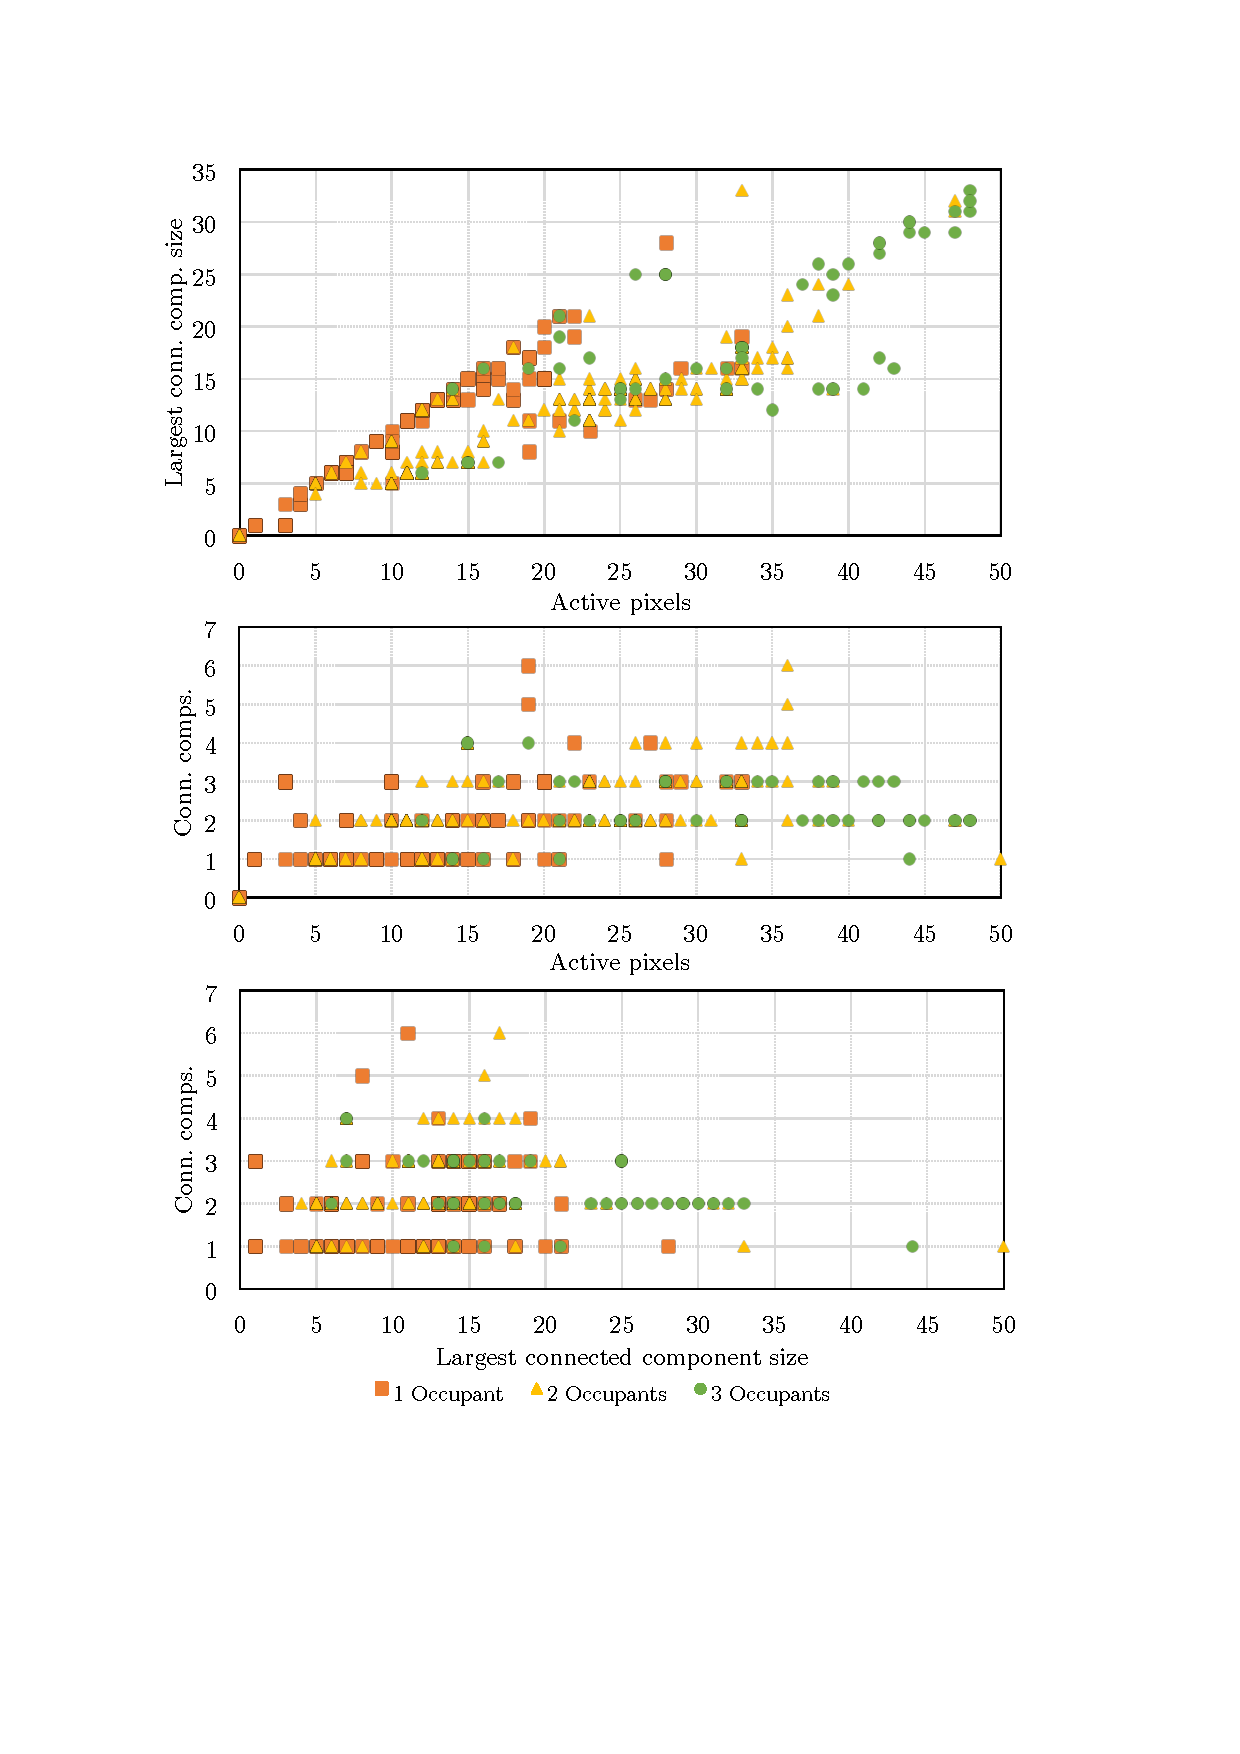
\includegraphics[width=0.93\textwidth]{../diagrams/feature-plots.pdf}
\caption{Plot of three features against each other with occupancy truth values}
\label{fig:featplots}
\end{figure}

\begin{figure}
\centering
\begin{subfigure}[b]{0.90\textwidth}
\centering
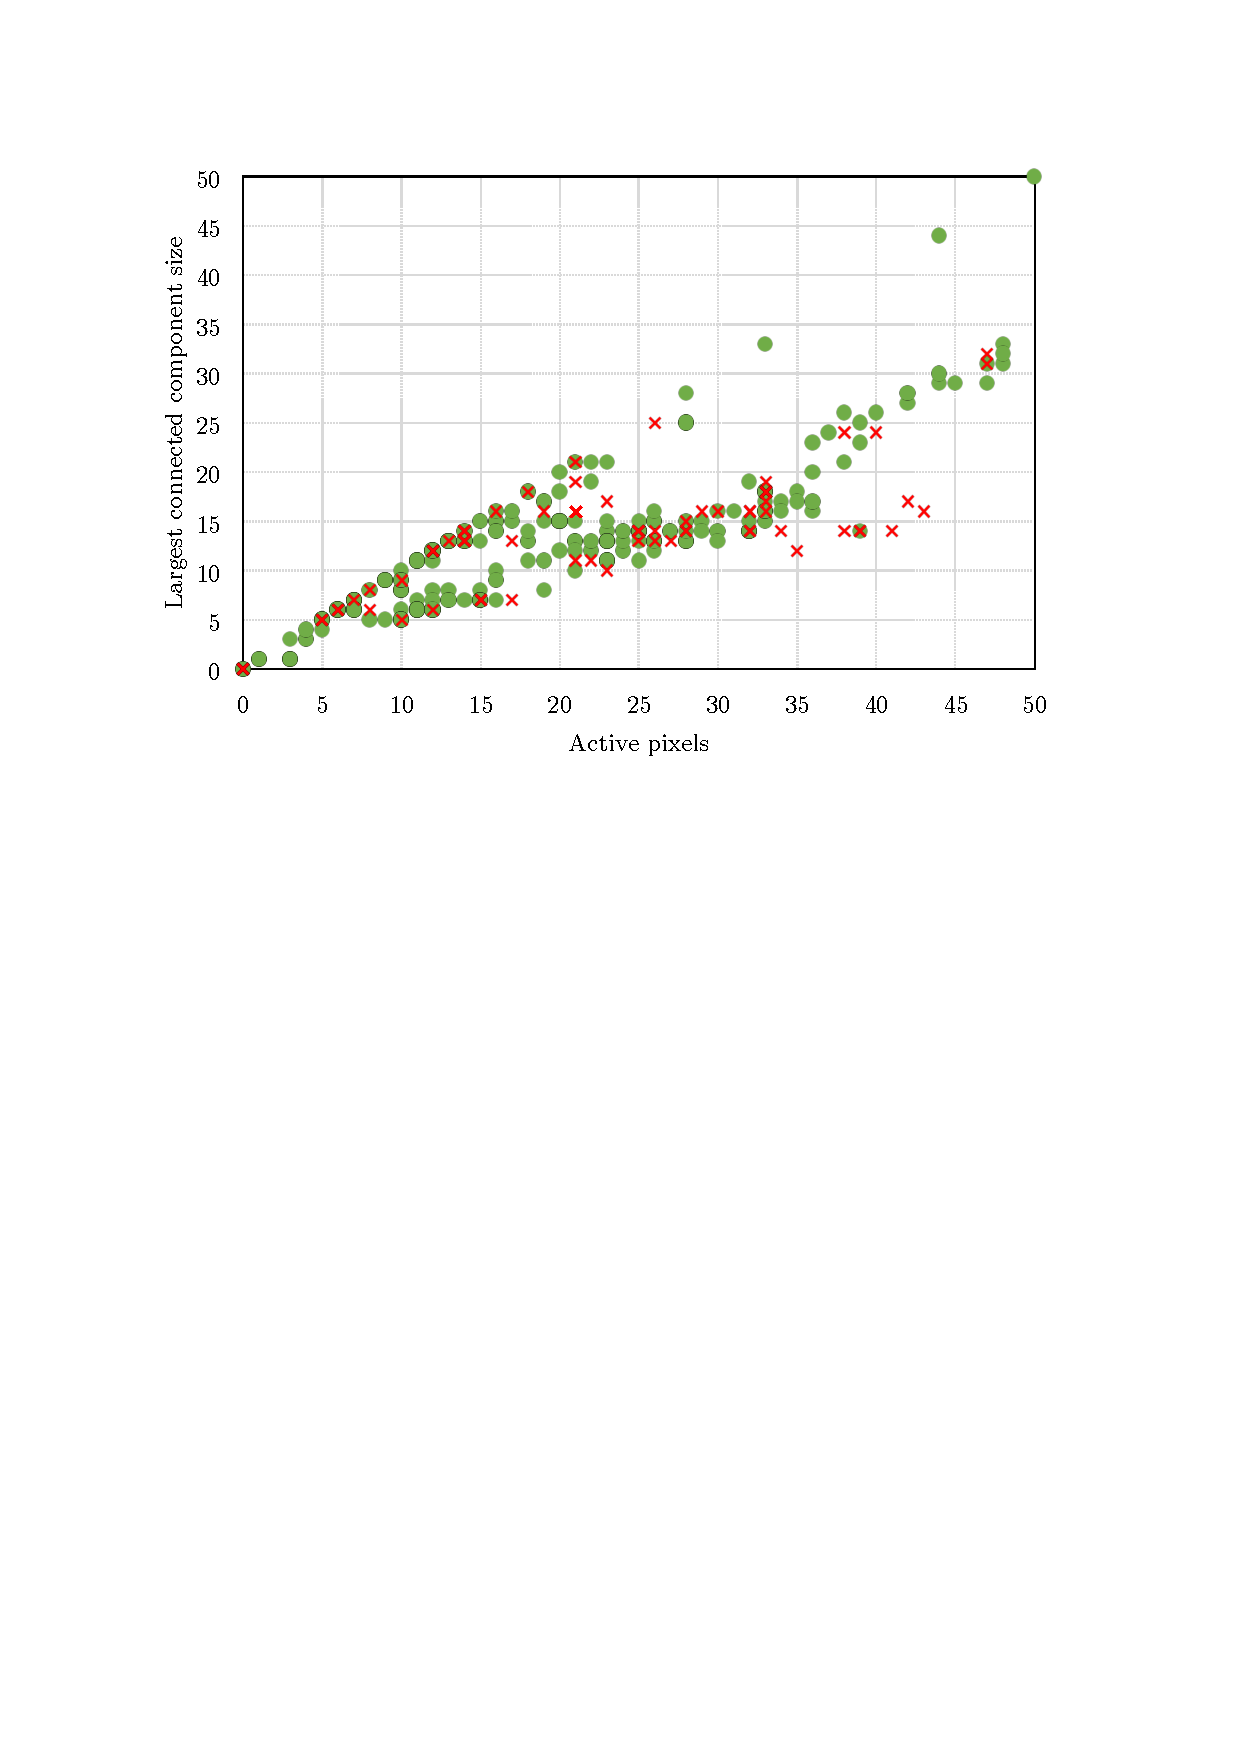
\includegraphics[width=\textwidth]{../diagrams/incorrect-correct-plot-kstar2.pdf}
\caption{K* Predictions, 82\% accurate}
\end{subfigure}

\begin{subfigure}[b]{0.90\textwidth}
\centering
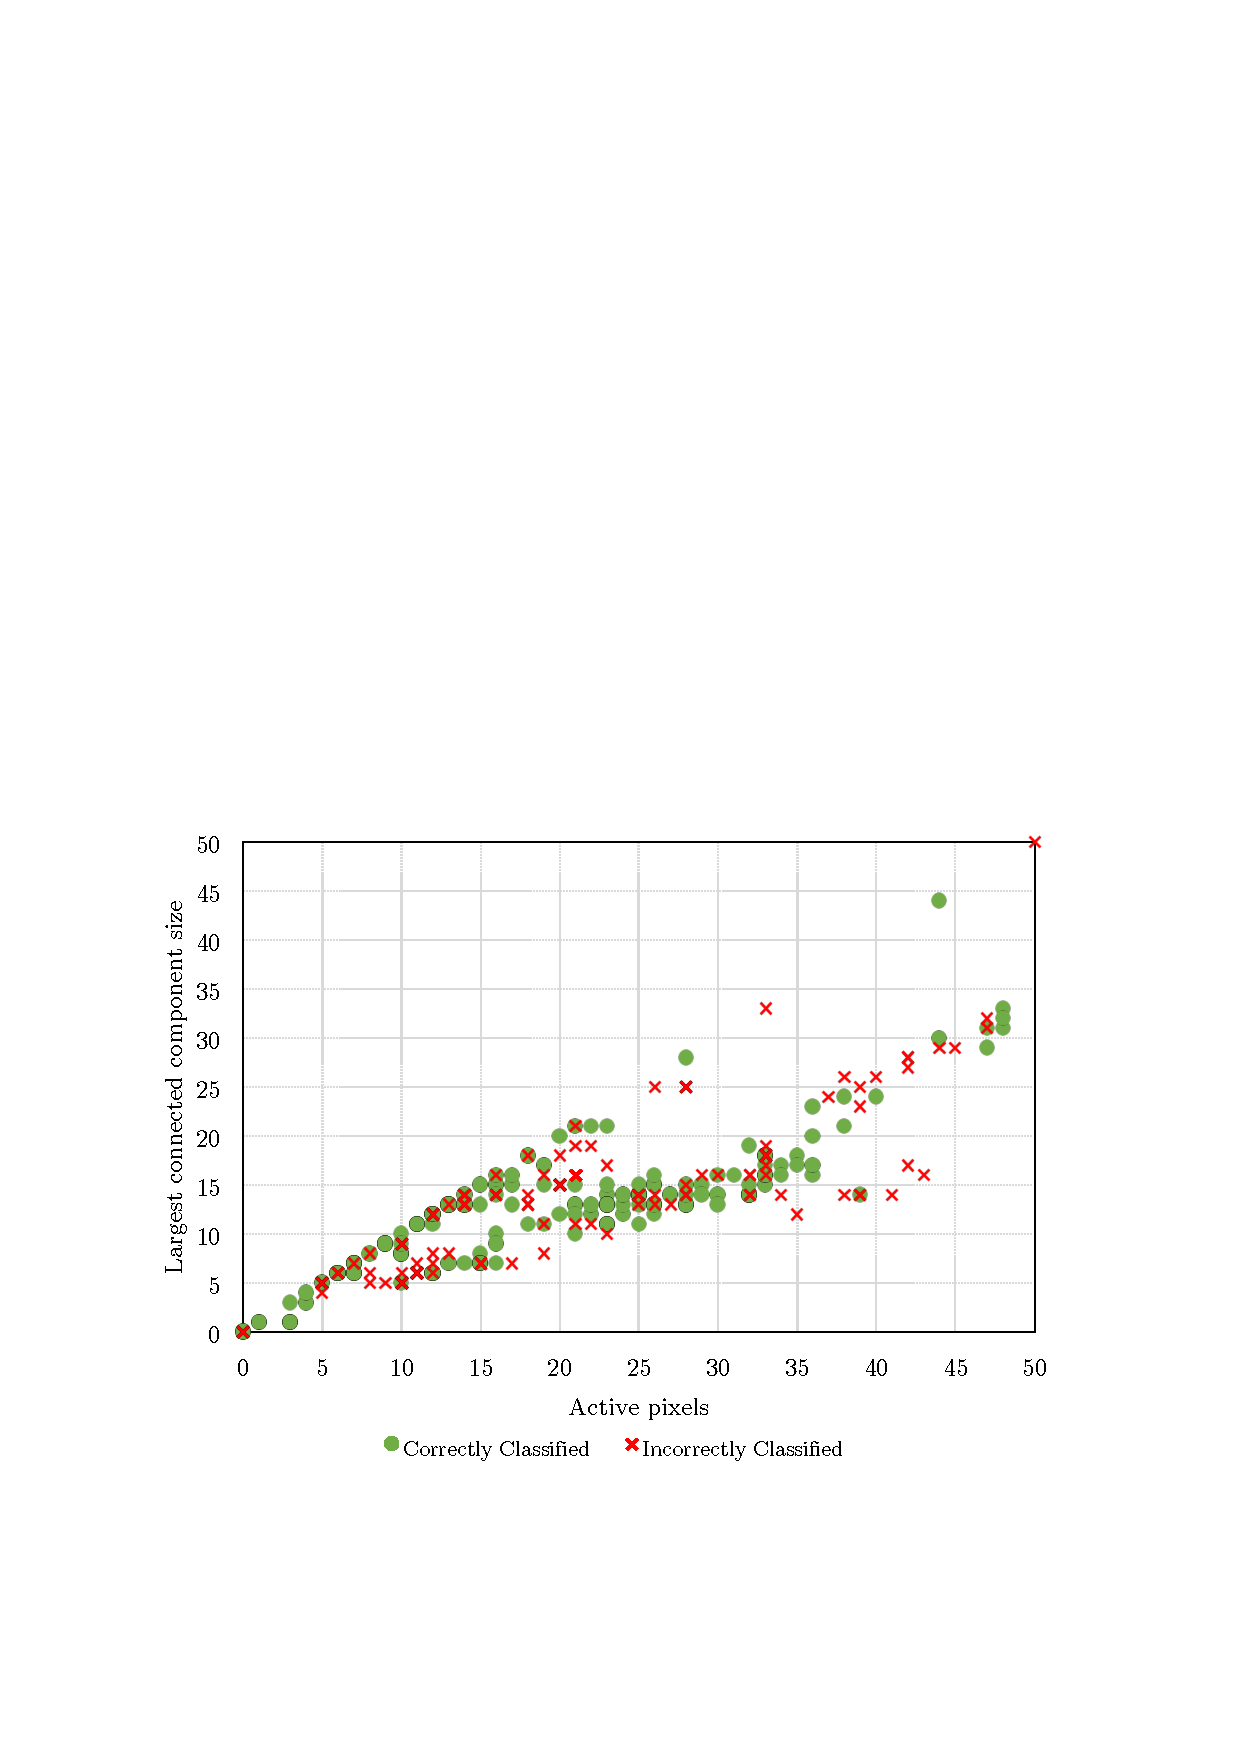
\includegraphics[width=\textwidth]{../diagrams/incorrect-correct-plot-smo2.pdf}
\caption{SVM Predictions, 67\% accurate}
\end{subfigure}
\caption{Plot of two feature vectors with different algorithms' predictions marked as correctly or incorrectly classified}
\label{fig:correctplots}
\end{figure}

\clearpage{}

\subsection{Energy Efficiency}
\begin{table}
\centering
\footnotesize
\renewcommand{\arraystretch}{1.2}
\begin{tabular}{l|r|r|r|r|r|r|r|r|}
\cline{2-9}
                                     & \textbf{Radio} & \textbf{Sleep} & \textbf{Wake} & \textbf{Volts} & \textbf{Wake} & \textbf{Sample} & \textbf{Avg}  & \textbf{Life}   \\ \cline{1-1}
\multicolumn{1}{|l|}{\textbf{Model}} &                & \textbf{(mA)}  & \textbf{(mA)} & \textbf{(V)}   & \textbf{(ms)} & \textbf{(Hz)}   & \textbf{(mW)} & \textbf{(days)} \\ \hline
\multicolumn{1}{|l|}{Existing}       & {\normalsize \xmark}  & {\normalsize 34}  & {\normalsize 52}  & {\normalsize 4.9}  & {\normalsize $\infty$}  & {\normalsize 0.20}  & {\normalsize 255.84}  & {\normalsize 8}   \\ \hline
\multicolumn{1}{|l|}{Sleep}          & {\normalsize \xmark}  & {\normalsize 34}  & {\normalsize 52}  & {\normalsize 4.9}  & {\normalsize 100}       & {\normalsize 0.20}  & {\normalsize 169.05}  & {\normalsize 12}  \\ \hline
\multicolumn{1}{|l|}{ThermoS.}       & {\normalsize \cmark}  & {\normalsize ?}   & {\normalsize ?}   & {\normalsize 3.3}  & {\normalsize ?}         & {\normalsize 0.20}  & {\normalsize 15.91}   & {\normalsize 131} \\ \hline
\multicolumn{1}{|l|}{LowPwr A}       & {\normalsize \cmark}  & {\normalsize 0.065} & {\normalsize 23}  & {\normalsize 3.3} & {\normalsize 300}  & {\normalsize 0.20} & {\normalsize 4.76}  & {\normalsize 438}    \\ \hline
\multicolumn{1}{|l|}{LowPwr B}       & {\normalsize \cmark}  & {\normalsize 0.065} & {\normalsize 23}  & {\normalsize 3.3} & {\normalsize 300}  & {\normalsize 0.01} & {\normalsize 0.44}  & {\normalsize 4718}   \\ \hline
\end{tabular}
\parbox{270pt}{
\vspace*{-13px}
{\footnotesize
\begin{tabbing}
Radio: ~~~~~~~~~~~~\= Does the model use radio transmission?\\
Sleep (mA): \> Milliamp current consumption in sleep state\\
Wake (mA): \> Milliamp current consumption in wake state\\
Volts (V): \> Voltage requirement of model\\
Wake (ms): \> Min. millisecond time model must be awake to sample \& transmit once\\
           \> ($\infty$ = never sleeps)\\
Sample (Hz): \> Freq. that model wakes and performs sample \& transmit\\
Avg (mW): \> Avg. milliwatt power given sleep/wake current, voltage, sample and wake time\\
Life (days): \> Est. life of model assuming a perfect 50~watt-hour~(Wh) battery
\end{tabbing}}}
\vspace*{-20px}
\caption{Comparison of different systems power consumption and their various energy efficiency traits}
\label{tab:lives}
\end{table}

As discussed in \fref{subsec:energy}, the prototype initially appears comparatively power hungry, as the ThermoSense system reported a power consumption of $\sim$4.8~mA, approximately $10\times$ less. However, making fair comparisons is difficult, as their data is incomplete. The 4.8~mA figure they quote is an average consumption figure taking into account all aspects of the wake/sleep cycle. No breakdown on wake times, sleep or wake current was provided, making direct comparisons on those metrics difficult. We examined the datasheets of their components and estimate a voltage of 3.3~V to generate our average milliwatt figure.

For our prototype sensing system, we restricted our adherence to low-power consumption to an architectural level, rather than making specific hardware and software changes. For our comparisons, we have elected to use a 50~watt-hour~(Wh) battery as a measure, as there exist inexpensive batteries in that class weighing around 300~grams \cite{AdafruitBattery} that provide a good balance between capacity and weight. We propose several different prototype designs in \Fref{tab:lives} and calculate theoretical prototype lifetimes assuming a perfect 50~Wh battery.

ThermoSense indicated that for each of their nodes, which consumed approximately 4.8~mA each, there were two 3~(Ah) batteries running in series. They indicated that at a sample rate of 0.2~Hz (once every 5 seconds) their prototype was able to run for approximately 21~days. Using our 50~Wh battery (``ThermoS.'' in \Fref{tab:lives}), we estimate that this would increase to approximately 131~days.

Our current prototype (``Existing'' in \Fref{tab:lives}) can boot and take one measure in approximately 100~ms, indicating it would need to be awake for 2\% of each five second window to perform one sample. Without any sleep, this prototype is always drawing a constant 52~mA, and consequently can only last 8~days.

If we were to implement a simple software-driven sleep cycle (``Sleep'' in \Fref{tab:lives}) minor power savings would occur. Incorporating sleep would reduce average current to 34~mA, assuming our present Arduino current draw. With the same battery capacity, we would expect battery life to increase to 12~days.

The high power consumption of our prototype is largely due to the use of off-the-shelf Arduino hardware which is not designed for low-power applications. Firstly, there exist several unnecessary LEDs that are constantly powered which could account for several milliamps. Secondly, there is a large power loss in our level shifting and voltage conversion circuit. We estimate that the resistors alone could be responsible for 3--4~mA of lost current. This is primarily a result of the 5~V, 3.3~V or 2.6~V requirements of different components. Standardizing the voltage at 3.3~V would allow several inefficient conversion circuits to be removed.

Contemplating a more real-world prototype, there exist Arduino boards that use the same processor as ours (and thereby are fully compatible) that can be constructed easily and reduce base power consumption to 7~mA, without sleep. In sleep mode, the power consumption drops to an impressive 43~\textmu A. A commonly used radio used in such devices is the ZigBee. Dementyev, Hodges and Taylor~\etal~\cite{dementyev2013power} suggest that a ZigBee radio would consume approximately 4.2~\textmu A when sleeping and 9.3~mA when awake, with a minimum wake time of around 270~ms to connect to the other nodes on the network. With a minimum data transfer rate of 20~kb/s and approximately 200 bytes of data to transmit each interval, we can set the upper limit of the radio wake time to be 300~ms. Using this radio, board and eliminating our voltage conversion issues (``LowPwr A'' in \Fref{tab:lives}) would increase the prototype's lifetime to around 438~days, a significant improvement over ThermoSense.

Additionally, in a real-world system, we contend that a sample rate of 0.01~Hz (once per 100 seconds) would provide sufficiently up-to-date information. Doing so provides an order of magnitude more battery life (``LowPwr B'' in \Fref{tab:lives}), with it being able to last more than 12~years.

Realistically, the battery lives of any of these prototypes would be less than estimated due to our assumptions about perfect efficiency, including the fact that an average battery would rarely hold its full charge for the time-scales discussed. However, these calculations provide us with useful relative comparative power and demonstrate that our prototype has the potential to be competitive with or better than ThermoSense in the realm of energy efficiency.

  \ifcsdef{mainfile}{}{\bibliography{../references/primary}}
\end{document}
 